\section{Introduction}
\label{sec:intro}
% object detection, video object detection
\begin{figure}
    \centering
    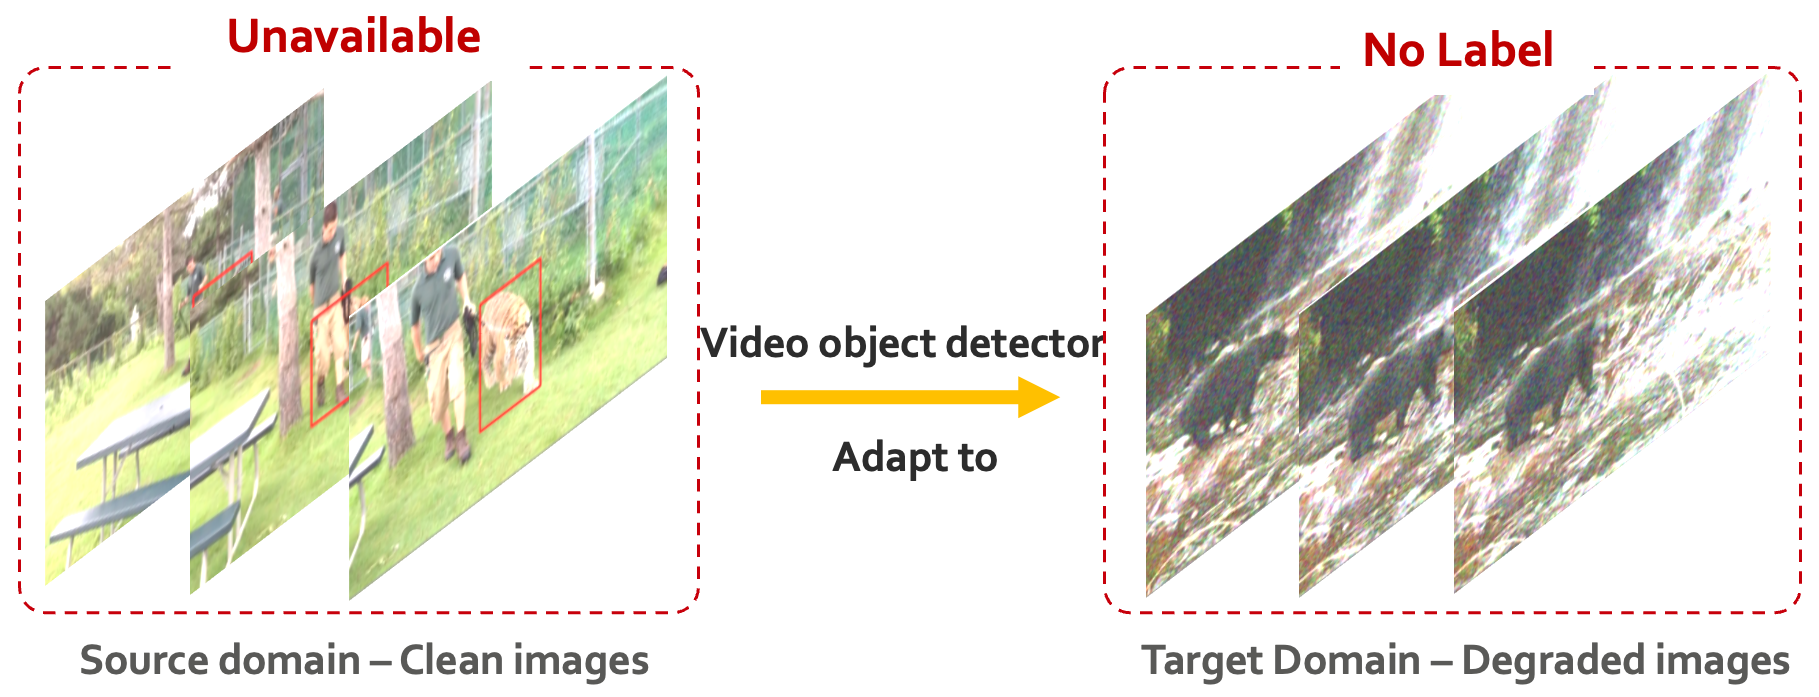
\includegraphics[width = 0.95\linewidth]{figures/overview.png}
    \caption{The scope of this work: we aim to adapt the video object detection model trained on clean image sequences to degraded image sequences under the condition that the data from the source domain and ground truth labels of the target domain are unavailable during the adaptation.}
    \label{fig:overview}
\end{figure}

Object detection in images and videos represents a pivotal task in computer vision, primarily owing to its extensive range of applications across diverse scenarios, such as intelligent surveillance systems and automated driving vehicles. Video object detection (VOD) aims to predict the bounding box and category information of all targeting objects in all video frames. Compared to single-frame object detection tasks, VOD enjoys the advantage of accessing additional information from the temporal dimension \cite{zhu2017flow, shi2023yolov}, which often contains consistent semantics and multiple views of the same target to help enrich the feature space and facilitate superior performance.  


% SFDA for object detection and our idea
When deploying object detectors in real-world settings, adverse imaging conditions caused by rain, haze, low light, or air turbulence often lead to a notable domain gap. These adverse conditions frequently result in a significant reduction in performance, underscoring the necessity for domain adaptation to bridge the gap. Typical domain adaptation (DA) methods require access to data and labels in both source and target domains, with labels in the target domain being relatively scarce \cite{adp_vp}. Due to the prohibitive cost of labeling target domain data, unsupervised domain adaptation (UDA) is sometimes required to facilitate effective fine-tuning on the target domain without any labels \cite{oza2023unsupervised}. In most DA and UDA cases for image detection, source domain data is provided to serve as anchors for adaptation. However, in some UDA scenarios, source data may not be available due to storage or privacy constraints, necessitating the optimization of detection networks under such limitations. To address this challenge, source-free domain adaptation (SFDA) is gaining increasing attention in the field of object detection, as it enables adaptation to target domains without relying on source domain data. 

\begin{figure*}
    \centering
    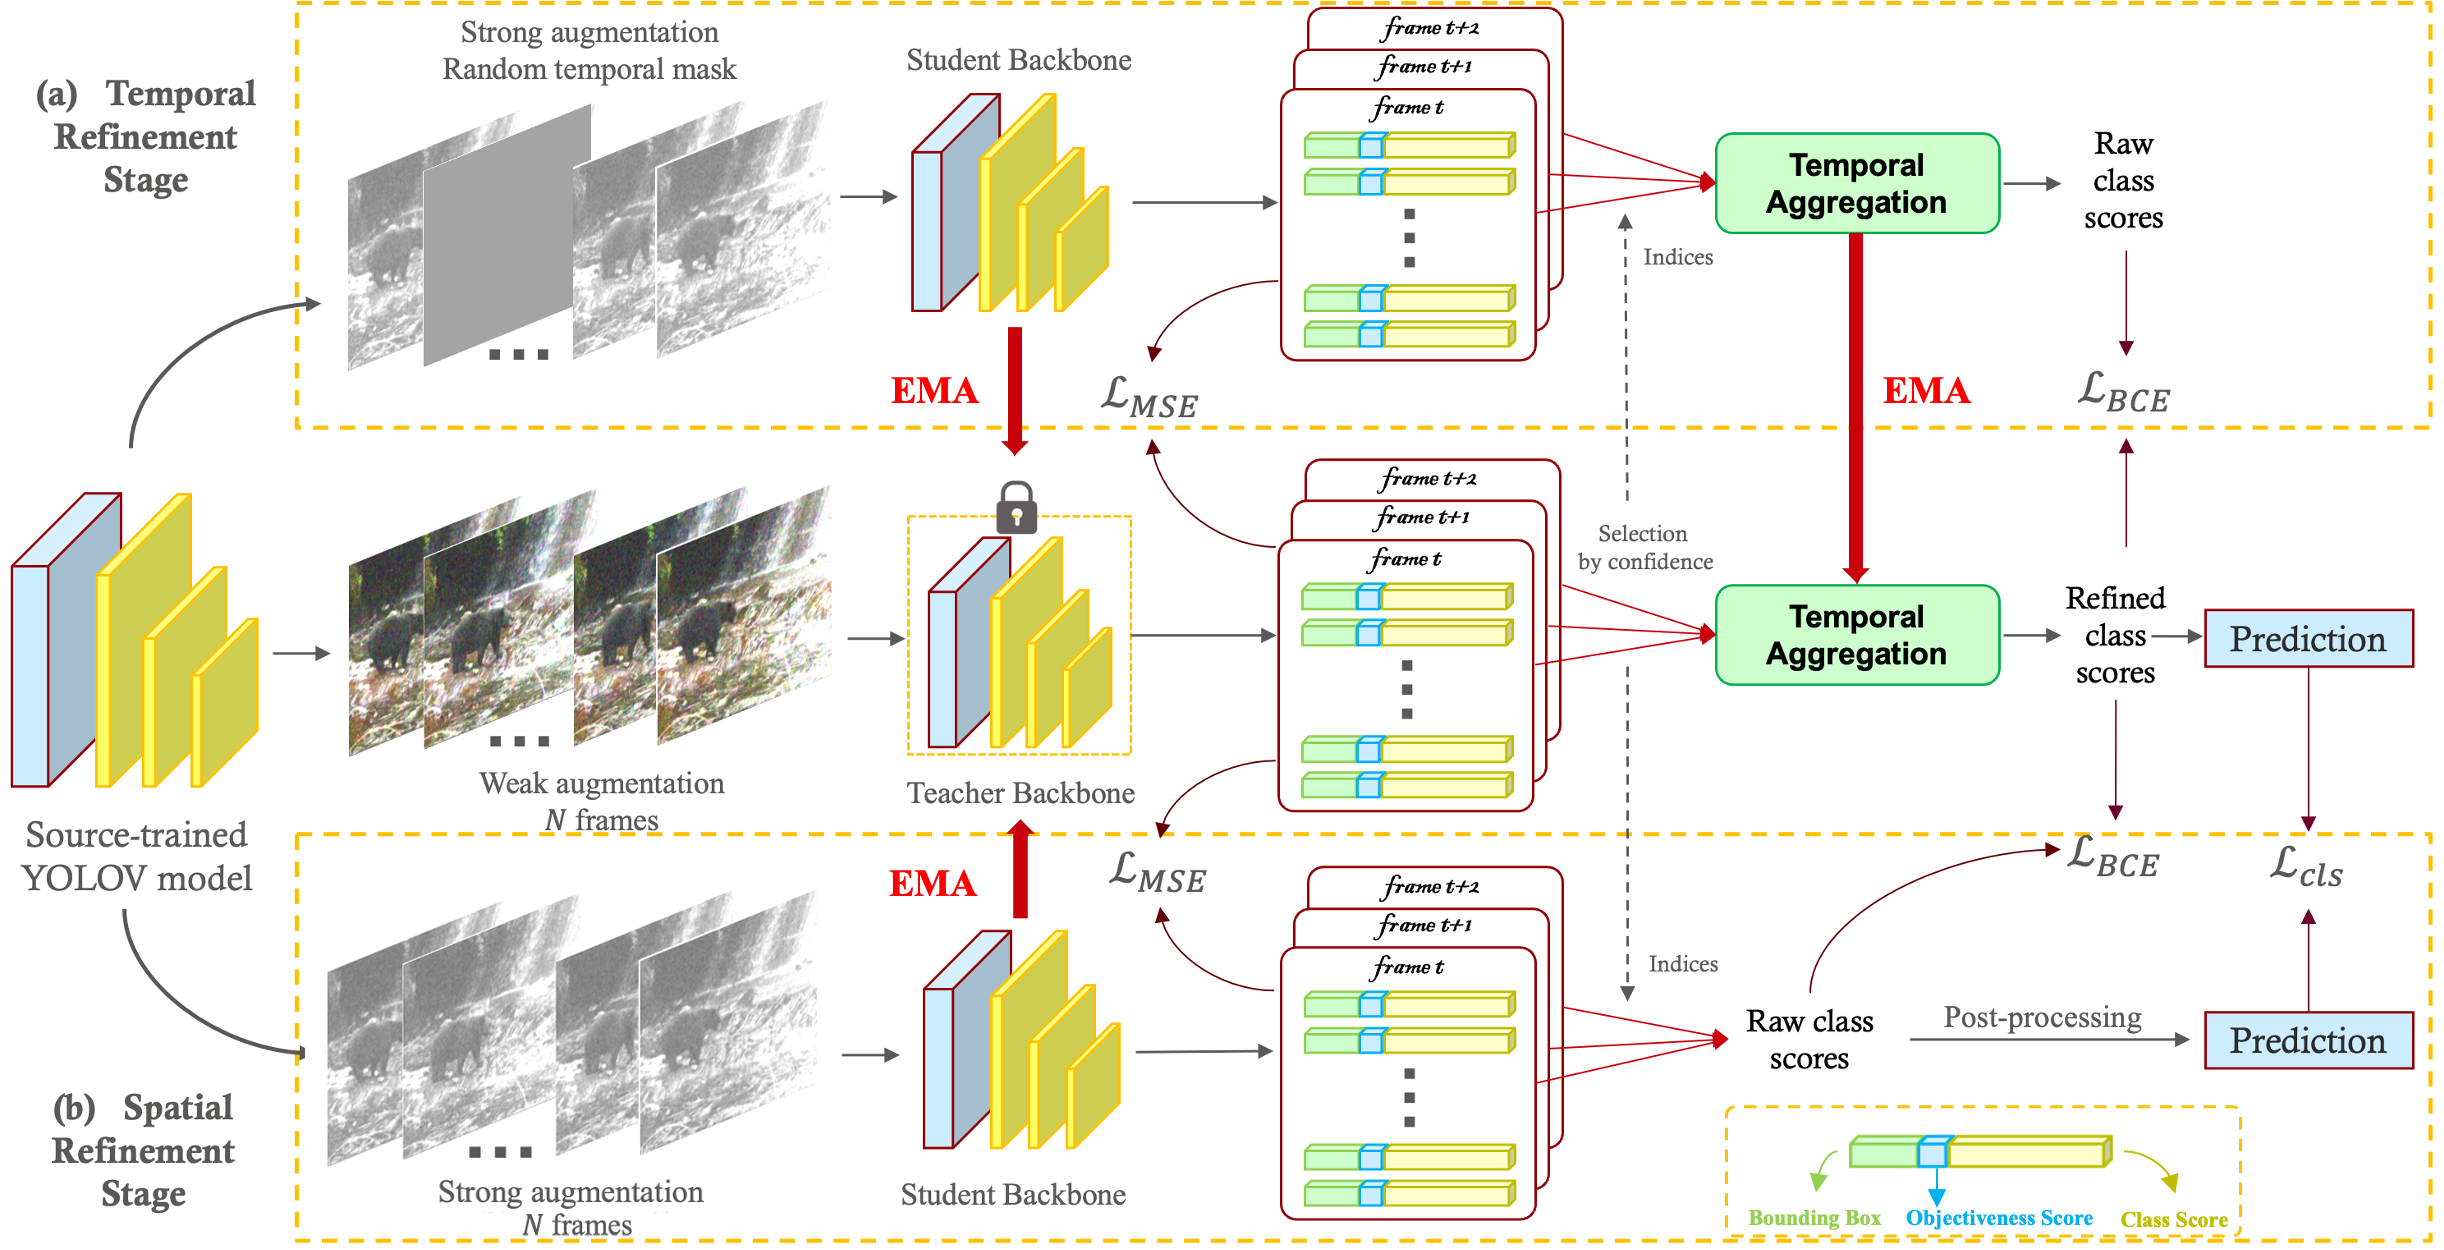
\includegraphics[width = 0.95\linewidth]{figures/SFVOD.png}
    \caption{Overview of the proposed STAR-MT for source-free adaptive video object detection. The domain adaptive fine-tuning alternately operates in two stages: (a) Temporal Refinement Stage (TRS) and (b) Spatial Refinement Stage (SRS).}
    \label{fig:SFVOD}
\end{figure*}

Although multiple approaches, such as those proposed in \cite{vibashan2023instance, li2022source, run_and_chase, chen2023exploiting, liu2023periodically, li2021free, cao2023contrastive}, have been developed recently to address SFDA for object detection, they predominantly focus on two-stage object detectors \cite{faster_rcnn}. To date, no prior work has specifically targeted SFDA for one-stage object detectors \cite{YOLOv1}, as their weights are more sensitive to fine-tuning, and intermediate features are highly abstract. Moreover, no SFDA method has been proposed for the video object detection task, primarily due to the scarcity of cross-domain video object detection datasets. However, given the unsupervised nature of SFDA, it is possible to explore source-free domain adaptation methods for video object detection using synthetic data. The scope of this work is illustrated in Fig. \ref{fig:overview}. One can expect those methods to be reliably applied to real-world scenarios where source domain data may not be readily available or accessible.

In this paper, we conduct analysis and experiments about basic SFDA techniques for the video object detection task and propose a novel SFDA method for the one-stage video object detector YOLOV \cite{shi2023yolov}. Specifically, we aim to adapt YOLOV \cite{shi2023yolov} to challenging adverse image conditions by alternately fine-tuning the video object detection model in the teacher-student learning framework. We summarize the contributions of this paper as follows:
% Inspired by YOLOV \cite{shi2023yolov} that leverages YOLOX \cite{ge2021yolox} to video object detection using robust temporal aggregation, we propose to use the temporally augmented predictions as pseudo labels to guide the fine-tuning of single-frame detector backbone in a mean-teacher scheme. 
\begin{itemize}
    \item We conduct the pioneering study exploring source-free unsupervised domain adaptation for video object detection (VOD). Specifically, we aim to adapt the YOLOV detector to adverse image conditions.
    \item We introduce a novel SFDA algorithm for VOD, termed Spatial-Temporal Alternate Refinement with Mean Teacher (STAR-MT). It alternately trains in two stages: the Temporal Refinement Stage works in a traditional mean-teacher learning scheme, while the Spatial Refinement Stage leverages temporally enhanced features to guide the single-frame backbone module. 
    \item We demonstrate the effectiveness of our method through experiments on different synthetic adverse image conditions, including noise, air turbulence, and haze. Given its unsupervised nature, STAR-MT is anticipated to yield reliable performance boost for video object detectors in real-world and unseen scenarios.

\end{itemize}
